\documentclass[12pt,a4paper]{article}
\usepackage[utf8]{inputenc} % inutile avec XeLaTeX/LuaLaTeX
\usepackage[T1]{fontenc}
\usepackage{amsmath,amssymb,mathrsfs,tikz,times,pifont}
\usepackage{enumitem}
\usepackage{multicol}
\usepackage{lmodern}
\newcommand\circitem[1]{%
\tikz[baseline=(char.base)]{
\node[circle,draw=gray, fill=red!55,
minimum size=1.2em,inner sep=0] (char) {#1};}}
\newcommand\boxitem[1]{%
\tikz[baseline=(char.base)]{
\node[fill=cyan,
minimum size=1.2em,inner sep=0] (char) {#1};}}
\setlist[enumerate,1]{label=\protect\circitem{\arabic*}}
\setlist[enumerate,2]{label=\protect\boxitem{\alph*}}
\everymath{\displaystyle}
\usepackage[left=1cm,right=1cm,top=1cm,bottom=1.7cm]{geometry}
\usepackage[colorlinks=true, linkcolor=blue, urlcolor=blue, citecolor=blue]{hyperref}
\usepackage{array,multirow}
\usepackage[most]{tcolorbox}
\usepackage{varwidth}
\usepackage{float}
\tcbuselibrary{skins,hooks}
\usetikzlibrary{patterns}

\usepackage{pgfplots}
\pgfplotsset{compat=1.15}
\usepackage{mathrsfs}
\usepackage{xcolor}  % Pour \color et \fcolorbox
\usepackage{amsmath}
\usepackage{amsfonts}
\usepackage{amssymb}
\usepackage{tkz-tab}
\usepackage{mdframed}
\usepackage{tikz}
\usetikzlibrary{arrows, shapes.geometric, fit}

% Commande pour la couleur d'accentuation
\newcommand{\myul}[2][black]{\setulcolor{#1}\ul{#2}\setulcolor{black}}
\newcommand\tab[1][1cm]{\hspace*{#1}}

%\usepackage[margin=2cm]{geometry}
\usepackage{eso-pic}         % Pour ajouter des éléments en arrière-plan

\usepackage{enumitem}
%---------------------------------------
% Définir un compteur pour les exemples
\newcounter{exemple}

% Définir la commande \exemple pour afficher un exemple numéroté
\newcommand{\exemple}{%
  \refstepcounter{exemple}% Incrémenter le compteur
  \textbf{\textcolor{orange}{Exemple \theexemple : }} \ignorespaces
}
%---------------------------------------
\newcounter{solution}

% Définir la commande \solutione pour afficher un solution numéroté
\newcommand{\solution}{%
  \refstepcounter{solution}% Incrémenter le compteur
  \textbf{\textcolor{orange}{Solution \thesolution : }} \ignorespaces
}
%---------------------------------------
\definecolor{myorange}{rgb}{1.0, 0.8, 0.0}

% Définir un compteur pour les exercices d'application
\newcounter{exerciceapp}

% Définir la commande pour afficher un exercice d'application numéroté
\newcommand{\exerciceapp}{%
  \refstepcounter{exerciceapp}%
  \textbf{\textcolor{myorange}{Exercice d'application \theexerciceapp :}} \ignorespaces
}
%--------------------------------------
% Définir un compteur pour les exercices d'application
\newcounter{correction}

% Définir la commande pour afficher un correction exercice d'application numéroté
\newcommand{\correction}{%
  \refstepcounter{correction}%
  \textbf{\textcolor{myorange}{Correction \thecorrection :}} \ignorespaces
}
%--------------------------------------
% Définir un compteur pour les remarque d'application
\newcounter{remarque}

%----------------------------------------
\definecolor{myorange1}{rgb}{1.0, 1.5, 0}
% Définir la commande pour afficher un remarque numéroté
\newcommand{\remarque}{%
  \refstepcounter{remarque}%
  \textbf{\textcolor{myorange1}{Remarque \theremarque :}} \ignorespaces
}

% Commande pour ajouter du texte en arrière-plan
\AddToShipoutPicture{
    \AtTextCenter{%
        \makebox[0pt]{\rotatebox{45}{\textcolor[gray]{0.6}{\fontsize{5cm}{5cm}\selectfont PGB}}}
    }
}

\begin{document}
% En-tête personnalisée
\begin{center}
    \Large\textbf{\underline{\textcolor{red}{Répérage}}}\\[-0.1cm]
    \normalsize\textbf{Prof : M. BA} \hfill \textbf{Classe : 2ndS}\\[-0.1cm]
    \textbf{Année scolaire : 2025 -- 2026}
\end{center}

\begin{center}
    \fbox{
        \Large \textbf{Chapitre : Repérage Cartésien et Droite du Plan}
    }
\end{center}

\vspace{0.5cm}

\section*{\centering \underline{\color{red}I- Repérage cartésien}}
\subsection*{\centering \underline{\color{red}\sffamily 1- Repérage sur une droite}}

\subsubsection*{\centering \underline{\color{red}a) Définition}}

Un repère sur une droite $(D)$ est un bipoint $(O, I)$ de $(D)$ tq $O \neq I$. \\
La distance $OI$ est l'unité de mesure sur $(D)$. \\
Le vecteur $\vec{i} = \overrightarrow{OI}$ est le vecteur directeur de $(D)$.

\vspace{0.5cm}

% Représentation simplifiée de la figure
\begin{center}
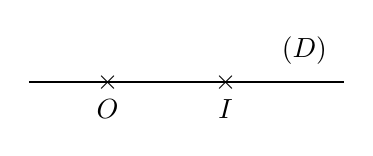
\begin{tikzpicture}[x=1cm, y=1cm]
    % Droite (D)
    \draw[thick] (-1,0) -- (3,0);
    \node[anchor=south] at (2.5, 0.1) {$(D)$};
    
    % Point O
    \node at (0,0) {$\times$};
    \node[anchor=north] at (0, -0.1) {$O$};
    
    % Point I
    \node at (1.5,0) {$\times$};
    \node[anchor=north] at (1.5, -0.1) {$I$};
\end{tikzpicture}
\end{center}

\subsubsection*{\centering \underline{\color{red}b) Abscisse d'un point}}

Soit $(D)$ une droite de vecteur directeur $\vec{i}$ et $O$ un point de $(D)$.

\begin{center}
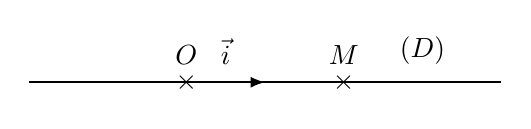
\begin{tikzpicture}[x=1cm, y=1cm]
    % La droite (D)
    \draw[thick] (-1,0) -- (5,0);
    
    % Point O
    \node at (1,0) {$\times$};
    \node[anchor=south] at (1, 0.1) {$O$};

    % Le vecteur i (flèche noire surmontée de i)
    \draw[->, >=latex, thick] (1,0) -- (2,0);
    \node[anchor=south] at (1.5, 0.1) {$\vec{i}$};
    
    % Point B
    \node at (3,0) {$\times$};
    \node[anchor=south] at (3, 0.1) {$M$};
    
    % Label (D)
    \node[anchor=south] at (4, 0.1) {$(D)$};
\end{tikzpicture}
\end{center}
Pour tout point $M \in (D)$ les vecteurs $\overrightarrow{OM}$ et $\vec{i}$ sont colinéaires. Alors il existe un unique réel $x$ tel que $\overrightarrow{OM} = x\vec{i}$.

\begin{itemize}
    \item[\color{red}*] $(O, \vec{i})$ est un repère de $(D)$ d'origine $O$.
    \item[\color{red}*] $x$ est l'abscisse du point $M$ sur $(O, \vec{i})$ noté souvent $x_M$.
\end{itemize}

\subsection*{\centering \underline{\color{red}\sffamily 2- Mesure algébrique}}

\subsubsection*{\centering \underline{\color{red} a) Définition}}

Soit $(D)$ une droite de repère $(O, \vec{i})$, $A$ et $B$ deux points de $(D)$.

\begin{center}
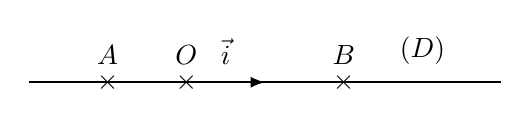
\begin{tikzpicture}[x=1cm, y=1cm]
    % La droite (D)
    \draw[thick] (-1,0) -- (5,0);
    
    % Point A
    \node at (0,0) {$\times$};
    \node[anchor=south] at (0, 0.1) {$A$};
    
    % Point O
    \node at (1,0) {$\times$};
    \node[anchor=south] at (1, 0.1) {$O$};

    % Le vecteur i (flèche noire surmontée de i)
    \draw[->, >=latex, thick] (1,0) -- (2,0);
    \node[anchor=south] at (1.5, 0.1) {$\vec{i}$};
    
    % Point B
    \node at (3,0) {$\times$};
    \node[anchor=south] at (3, 0.1) {$B$};
    
    % Label (D)
    \node[anchor=south] at (4, 0.1) {$(D)$};
\end{tikzpicture}
\end{center}

Les vecteurs $\overrightarrow{AB}$ et $\vec{i}$ sont colinéaires donc il existe un réel $K$ tel que $\overrightarrow{AB} = K\vec{i}$.

Le réel $K$ est appelé mesure algébrique du vecteur $\overrightarrow{AB}$ relativement à $\vec{i}$.

\subsubsection*{\centering \underline{\color{red}b) Notation}}

La mesure algébrique du vecteur $\overrightarrow{AB}$ est notée $\overline{AB}$ ($K = \overline{AB}$).

D'où $\overrightarrow{AB} = \overline{AB} \ \vec{i}$ et par conséquent, on a les propriétés suivantes.

\subsubsection*{\centering \underline{\color{red}c) Propriétés}}

\begin{itemize}
    \item[\color{red} i)] $|\overline{AB}| = AB$
    \item[\color{red} ii)] $\overline{BA} = -\overline{AB}$
    \item[\color{red} iii)] Lorsque $A \neq B$, on a :
    \[ \overline{AB} = \begin{cases} AB & \text{si } \overrightarrow{AB} \text{ et } \vec{i} \text{ sont colinéaires} \\ \text{ou} \\ -AB & \text{si } \overrightarrow{AB} \text{ et } \vec{i} \text{ sont de sens contraire} \end{cases} \]
    \item[\color{red} iv)] $\overline{AB} = 0 \iff A = B$
    \item[\color{red} v)] Pour tout $\lambda \in \mathbb{R}$, $\overrightarrow{AB} = \lambda \overrightarrow{AC} \iff \overline{AB} = \lambda \overline{AC}$
    \item[\color{red} vi)] $\overline{AC} = \overline{AB} + \overline{BC}$ (Relation de Chasles)
    \item[\color{red} vii)] $\overline{AB} = x_B - x_A$
\end{itemize}

\noindent \underline{\textbf{\color{red}Remarque :}} \\
Si $(O, I)$ est un repère axial d'une droite $(D)$ alors pour tout point $M \in (D)$, on a :
\[ x_M = \frac{\overline{OM}}{\overline{OI}} \]

\noindent \underline{\textbf{Exemple :}}

\begin{center}
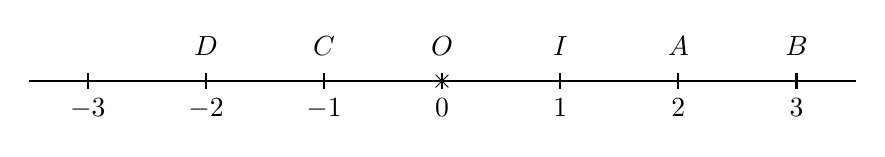
\begin{tikzpicture}[x=1.5cm, y=1cm]
    % Axe horizontal
    \draw[thick] (-3.5,0) -- (3.5,0);
    
    % Graduations et nombres
    \foreach \x in {-3,-2,-1,0,1,2,3} {
        \draw[thick] (\x,0.1) -- (\x,-0.1);
        \node[below] at (\x,-0.1) {$\x$};
    }
    
    % Points avec leurs labels au-dessus
    \node[anchor=south] at (-2, 0.2) {$D$};
    \node[anchor=south] at (-1, 0.2) {$C$};
    \node[anchor=south] at (0, 0.2) {$O$};
    \node at (0,0) {$\times$}; % O est marqué par une croix
    \node[anchor=south] at (1, 0.2) {$I$};
    \node[anchor=south] at (2, 0.2) {$A$};
    \node[anchor=south] at (3, 0.2) {$B$};
\end{tikzpicture}
\end{center}

\medskip

Dans le repère $(O, I)$ : $x_M = \dfrac{\overline{OM}}{\overline{OI}} \quad \forall M \in (D)$

\medskip

$x_A = \dfrac{\overline{OA}}{\overline{OI}} = \dfrac{2}{1} = 2$

\smallskip

$x_D = \dfrac{\overline{OD}}{\overline{OI}} = \dfrac{-2}{1} = -2$

\medskip

Dans le repère $(A, B)$ : $x_M = \dfrac{\overline{AM}}{\overline{AB}} \quad \forall M \in (D)$

\medskip

$x_A = \dfrac{\overline{AA}}{\overline{AB}} = \dfrac{0}{\overline{AB}} = 0$

\smallskip

$x_B = \dfrac{\overline{AB}}{\overline{AB}} = 1$

\smallskip

$x_D = \dfrac{\overline{AD}}{\overline{AB}} = \dfrac{x_D - x_A}{x_B - x_A} = \dfrac{-2 - 2}{3 - 2} = -4$

% --- 3- Version algébrique du Théorème de Thalès ---
\section*{\centering \underline{\color{red}3- Version algébrique du Théorème de Thalès et sa réciproque}}

\subsubsection*{\centering \underline{\color{red} a) Théorème de Thalès}}

Soit $ABC$ un triangle, $M$ un point de $(AB)$ et $N$ un point de $(AC)$. \\
Si $(MN) // (BC)$ alors $\dfrac{\overline{AM}}{\overline{AB}} = \dfrac{\overline{AN}}{\overline{AC}} = \dfrac{\overline{MN}}{\overline{BC}}$

\subsubsection*{\centering \underline{\color{red} b) Propriété réciproque}}


Soit $ABC$ un triangle, $M$ un point de $(AB)$ et $N$ un point de $(AC)$. \\
Si $\dfrac{\overline{AM}}{\overline{AB}} = \dfrac{\overline{AN}}{\overline{AC}}$ alors $(MN) // (BC)$

\subsubsection*{\centering \underline{\color{red} 4) Base du plan vectoriel}}
\subsubsection*{\centering \underline{\color{red} a) Définition}}

\vspace{0.3cm}

On appelle \textbf{base du plan vectoriel} tout couple {\color{red} $(\vec{i}, \vec{j})$} de vecteurs non colinéaires.

\vspace{0.2cm}

{\color{red} En particulier :}
\begin{itemize}
    \item[\color{red} i)] La base {\color{red} $(\vec{i}, \vec{j})$} est dite \textbf{base orthogonale} ssi {\color{red} $\vec{i} \perp \vec{j}$}
    \item[\color{red} ii)] La base {\color{red} $(\vec{i}, \vec{j})$} est dite \textbf{base orthonormale} (ou base orthonormé) ssi {\color{red} $\vec{i} \perp \vec{j}$} et {\color{red} $\|\vec{i}\| = \|\vec{j}\| = 1$}
\end{itemize}

\subsubsection*{\centering \underline{\color{red} Exemple :}}

Soit $ABC$ un triangle rectangle en $A$.

% Pour le triangle, tu peux utiliser l'environnement picture ou tikz si nécessaire
\begin{center}
    % [Schéma du triangle rectangle ABC ici]
\end{center}

{\color{red}$(\vec{BA}, \vec{BC})$} est une base car $\vec{BA}$ et $\vec{BC}$ sont non colinéaires. \\
{\color{red}$(\vec{AB}, \vec{AC})$} est une base orthogonale car {\color{red}$\vec{AB} \perp \vec{AC}$}.

\vspace{0.5cm}

\subsubsection*{\centering \underline{\color{red} b) Coordonnées d'un vecteur}}

Soit {\color{red}$(\vec{i}, \vec{j})$} une base du plan vectoriel. Pour tout vecteur {\color{red}$\vec{u}$} du plan, il existe un unique couple {\color{red}$(x, y)$} de réels tels que {\color{red}$\vec{u} = x\vec{i} + y\vec{j}$}.

Les réels {\color{red}$x$} et {\color{red}$y$} sont les coordonnées du vecteur {\color{red}$\vec{u}$} dans la base {\color{red}$(\vec{i}, \vec{j})$} et on note {\color{red}$\vec{u} \begin{pmatrix} x \\ y \end{pmatrix}$} (ou bien {\color{red}$\vec{u}(x, y)$}).

\subsubsection*{\centering \underline{\color{red} c) Condition de colinéarité}}
\subsubsection*{\centering \underline{\color{red} Définition}}

\vspace{0.3cm}

Soient {\color{red}$\vec{u} \begin{pmatrix} x \\ y \end{pmatrix}$} et {\color{red}$\vec{v} \begin{pmatrix} x' \\ y' \end{pmatrix}$} deux vecteurs du plan. On appelle déterminant de {\color{red}$(\vec{u}, \vec{v})$} noté {\color{red}$det(\vec{u}, \vec{v})$}, le réel défini par :

\vspace{0.2cm}

{\color{red} $det(\vec{u}, \vec{v}) = \begin{vmatrix} x & x' \\ y & y' \end{vmatrix} = xy' - x'y$}

\subsubsection*{\centering \underline{\color{red} Propriété :}}

Deux vecteurs {\color{red}$\vec{u} \begin{pmatrix} x \\ y \end{pmatrix}$} et {\color{red}$\vec{v} \begin{pmatrix} x' \\ y' \end{pmatrix}$} sont colinéaires \\
ssi {\color{red}$det(\vec{u}, \vec{v}) = 0$} \\
ssi {\color{red}$xy' - x'y = 0$}

\vspace{0.3cm}

\textbf{\underline{\exerciceapp}}

Soit {\color{red}$(\vec{i}, \vec{j})$} une base du plan vectoriel. On considère les vecteurs {\color{red}$\vec{u}$} et {\color{red}$\vec{v}$} définis par :
\begin{center}
    {\color{red}$\vec{u} = 2\vec{i} - \vec{j}$} et {\color{red}$\vec{v} = \vec{i} + 3\vec{j}$}
\end{center}

1-a) Montrer que {\color{red}$(\vec{u}, \vec{v})$} est une base. \\
b) Exprimer {\color{red}$\vec{i}$} et {\color{red}$\vec{j}$} en fonction de {\color{red}$\vec{u}$} et {\color{red}$\vec{v}$} puis donner les coordonnées de {\color{red}$\vec{i}$} et {\color{red}$\vec{j}$} dans la base {\color{red}$(\vec{u}, \vec{v})$}.

2) Soit {\color{red}$\vec{w}$} de coordonnées {\color{red}$(x, y)$} dans la base {\color{red}$(\vec{u}, \vec{v})$}. Déterminer les coordonnées de {\color{red}$\vec{w}$} dans la base {\color{red}$(\vec{i}, \vec{j})$}.

3) Soit {\color{red}$\vec{n} = \alpha\vec{i} + \beta\vec{j}$}, où {\color{red}$\alpha, \beta \in \mathbb{R}$}. \\
Déterminer les coordonnées de {\color{red}$\vec{n}$} dans la base {\color{red}$(\vec{u}, \vec{v})$}.

4) Application : Soit $P$ de coordonnées {\color{red}$(-1, 3)$}. \\
Déterminer les coordonnées de $P$ dans {\color{red}$(\vec{u}, \vec{v})$}.

\subsubsection*{\centering \underline{\color{red} 5) Repère du plan}}
\subsubsection*{\centering \underline{\color{red} a) Définition}}

\vspace{0.3cm}

On appelle repère cartésien du plan tout triplet {\color{red}$(O, \vec{i}, \vec{j})$} tel que {\color{red}$O$} est un point et {\color{red}$(\vec{i}, \vec{j})$} est une base. \\
Le point {\color{red}$O$} est appelé origine du repère.

\vspace{0.2cm}

{\color{red} En particulier :}
\begin{itemize}
    \item[\color{red} i)] Le repère {\color{red}$(O, \vec{i}, \vec{j})$} est dit orthogonal ssi la base {\color{red}$(\vec{i}, \vec{j})$} est orthogonale ({\color{red}$\vec{i} \perp \vec{j}$}).
    \item[\color{red} ii)] Le repère {\color{red}$(O, \vec{i}, \vec{j})$} est dit orthonormé ou orthonormal ssi la base {\color{red}$(\vec{i}, \vec{j})$} est orthogonale ({\color{red}$\vec{i} \perp \vec{j}$}) et {\color{red}$\|\vec{i}\| = \|\vec{j}\| = 1$}.
\end{itemize}

\subsubsection*{\centering \underline{\color{red} b) Coordonnées d'un point dans le plan}}


Soit \textcolor{red}{$(O, \vec{i}, \vec{j})$} un repère du plan. Alors pour tout point \textcolor{red}{$M$} du plan, il existe un unique couple \textcolor{red}{$(x, y)$} de réels tels que :
\(
\color{red}{\overrightarrow{OM} = x\vec{i} + y\vec{j}}
\)

Les réels $x$ et $y$ sont appelés \textbf{coordonnées du point $M$} et on note $\color{red}{M \begin{pmatrix} x \\ y \end{pmatrix}}$ ou $\color{red}{M(x, y)}$.

\noindent \underline{\textcolor{red}{Remarque : Repère affine}} \\
Tous les points $A, B, C$ non alignés du plan forment un repère $(A, B, C)$ ou $(A, \overrightarrow{AB}, \overrightarrow{AC})$ appelé repère affine dans lequel on a : 
$A \begin{pmatrix} 0 \\ 0 \end{pmatrix}$, $B \begin{pmatrix} 1 \\ 0 \end{pmatrix}$, $C \begin{pmatrix} 0 \\ 1 \end{pmatrix}$

\noindent \underline{\textcolor{red}{Exemple :}} Soit $ABC$ un triangle.

\begin{center}
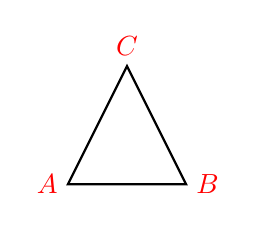
\begin{tikzpicture}[scale=1.5]
    \coordinate (A) at (0,1);
    \coordinate (B) at (1,0);
    \coordinate (C) at (0.5,1.5);
    \draw[thick] (0,0) node[left]{\textcolor{red}{$A$}} -- (1,0) node[right]{\textcolor{red}{$B$}} -- (0.5,1) node[above]{\textcolor{red}{$C$}} -- cycle;
\end{tikzpicture}
\end{center}

\noindent Dans le repère $(B, A, C)$ : $B \begin{pmatrix} 0 \\ 0 \end{pmatrix}$ ; $A \begin{pmatrix} 1 \\ 0 \end{pmatrix}$ ; $C \begin{pmatrix} 0 \\ 1 \end{pmatrix}$ \\
\noindent Dans le repère $(C, B, A)$ : $C \begin{pmatrix} 0 \\ 0 \end{pmatrix}$ ; $B \begin{pmatrix} 1 \\ 0 \end{pmatrix}$ ; $A \begin{pmatrix} 0 \\ 1 \end{pmatrix}$

\subsubsection*{\centering \underline{\color{red}{c) Changement de repère par translation}}}

Soient {\color{red}$(O, \vec{i}, \vec{j})$} un repère du plan et {\color{red}$A \begin{pmatrix} x_A \\ y_A \end{pmatrix}$} dans {\color{red}$(O, \vec{i}, \vec{j})$}. \\
Soient {\color{red}$M \begin{pmatrix} x \\ y \end{pmatrix}$} dans {\color{red}$(O, \vec{i}, \vec{j})$} et {\color{red}$M \begin{pmatrix} X \\ Y \end{pmatrix}$} dans {\color{red}$(A, \vec{i}, \vec{j})$}.

$\overrightarrow{OM} = \overrightarrow{OA} + \overrightarrow{AM}$

$M \begin{pmatrix} x \\ y \end{pmatrix}$ dans $(O, \vec{i}, \vec{j}) \Rightarrow \overrightarrow{OM} = x\vec{i} + y\vec{j}$

$A \begin{pmatrix} x_A \\ y_A \end{pmatrix}$ dans $(O, \vec{i}, \vec{j}) \Rightarrow \overrightarrow{OA} = x_A\vec{i} + y_A\vec{j}$

$M \begin{pmatrix} X \\ Y \end{pmatrix}$ dans $(A, \vec{i}, \vec{j}) \Rightarrow \overrightarrow{AM} = X\vec{i} + Y\vec{j}$

Donc $x\vec{i} + y\vec{j} = (x_A\vec{i} + y_A\vec{j}) + (X\vec{i} + Y\vec{j})$ \\
\indent \enspace $x\vec{i} + y\vec{j} = (x_A + X)\vec{i} + (y_A + Y)\vec{j}$

Ainsi, on en déduit que :

\begin{center}
{\color{red}
$\begin{cases} x = x_A + X \\ y = y_A + Y \end{cases}$} 
\quad ou bien \quad 
{\color{red}
$\begin{cases} X = x - x_A \\ Y = y - y_A \end{cases}$}
\end{center}

\noindent \underline{\textcolor{red}{Théorème -- définition}} \\
Soient $A \begin{pmatrix} x_A \\ y_A \end{pmatrix}$ et $M \begin{pmatrix} x \\ y \end{pmatrix}$ dans un repère $(O, \vec{i}, \vec{j})$ et $M \begin{pmatrix} X \\ Y \end{pmatrix}$ dans le repère $(A, \vec{i}, \vec{j})$, alors :

\[
\fcolorbox{red}{white}{$ \begin{cases} X = x - x_A \\ Y = y - y_A \end{cases} $}
\]

Ce système est dit \textcolor{red}{formules de changement de repère}.

\noindent \underline{\textcolor{red}{Exemple :}} \\
Soit $A \begin{pmatrix} 1 \\ 2 \end{pmatrix}$ et $M \begin{pmatrix} -1 \\ 3 \end{pmatrix}$ dans un repère $(O, \vec{i}, \vec{j})$. Donner les coordonnées de $M$ dans le repère $(A, \vec{i}, \vec{j})$.

\noindent \underline{\textcolor{red}{Correction}} \\
Soit $M \begin{pmatrix} X \\ Y \end{pmatrix}$ dans $(A, \vec{i}, \vec{j})$ alors : 
$\begin{cases} X = x_M - x_A \\ Y = y_M - y_A \end{cases}$

$\begin{cases} X = -1 - 1 \\ Y = 3 - 2 \end{cases}$

$\begin{cases} X = -2 \\ Y = 1 \end{cases}$

\noindent Donc $M \begin{pmatrix} -2 \\ 1 \end{pmatrix}$ dans $(A, \vec{i}, \vec{j})$.

\section*{\centering \underline{\color{red}II -- Droite du plan}}
\subsection*{\centering \underline{\color{red}\sffamily 1- Détermination d'une droite}}

Une droite $(D)$ du plan peut être déterminée par :
\begin{itemize}
    \item[\textcolor{red}{--}] Deux points distincts de $(D)$
    \item[\textcolor{red}{--}] Ou bien par un point $A$ de $(D)$ et un vecteur directeur de $(D)$ non nul.
\end{itemize}

\subsubsection*{\underline{\textcolor{red}{a) Détermination d'une droite par deux points distincts}}}

Soient $(D)$ une droite du plan, \textcolor{red}{$A$ et $B$} deux points de $(D)$ tels que \textcolor{red}{$A \neq B$}.

Pour tout point $M \in (D)$, les vecteurs \textcolor{red}{$\overrightarrow{AM}$ et $\overrightarrow{AB}$} sont \textcolor{red}{colinéaires} et donc \textcolor{red}{$\det(\overrightarrow{AM}, \overrightarrow{AB}) = 0$}

\begin{center}
    \textcolor{red}{$\forall M \in (D) \Rightarrow \det(\overrightarrow{AM}, \overrightarrow{AB}) = 0$}
\end{center}

\noindent \underline{\textcolor{red}{Application}} \\
Soient $(O, \vec{i}, \vec{j})$ un repère du plan, $A \begin{pmatrix} 2 \\ 1 \end{pmatrix}$ et $B \begin{pmatrix} 1 \\ 2 \end{pmatrix}$ dans $(O, \vec{i}, \vec{j})$. \\
Déterminer l'équation de la droite $(D)$.

\begin{center}
    \underline{\textcolor{red}{Correction}}
\end{center}

\noindent Soit $M \begin{pmatrix} x \\ y \end{pmatrix} \in (D)$. Alors $\det(\overrightarrow{AM}, \overrightarrow{AB}) = 0$

$\overrightarrow{AM} \begin{pmatrix} x_M - x_A \\ y_M - y_A \end{pmatrix} \Rightarrow \overrightarrow{AM} \begin{pmatrix} x - 2 \\ y - 1 \end{pmatrix}$

$\overrightarrow{AB} \begin{pmatrix} x_B - x_A \\ y_B - y_A \end{pmatrix} \Rightarrow \overrightarrow{AB} \begin{pmatrix} -1 \\ 1 \end{pmatrix}$

$\det(\overrightarrow{AM}, \overrightarrow{AB}) = \begin{vmatrix} x - 2 & -1 \\ y - 1 & 1 \end{vmatrix}$

$\det(\overrightarrow{AM}, \overrightarrow{AB}) = (x - 2)(1) - (y - 1)(-1)$ \\
\indent \enspace \qquad \qquad $= x - 2 + y - 1$

$\det(\overrightarrow{AM}, \overrightarrow{AB}) = x + y - 3$

\noindent D'où $(D) : \boxed{x + y - 3 = 0}$

\subsubsection*{\underline{\textcolor{red}{b) Détermination d'une droite par un point et un vecteur directeur non nul}}}

Soit $(D)$ une droite, $A \in (D)$ et $\vec{u}$ un vecteur directeur non nul de $(D)$. Alors pour tout $M \in (D)$, \textcolor{red}{$\overrightarrow{AM}$ et $\vec{u}$} sont \textcolor{red}{colinéaires}, et donc \textcolor{red}{$\det(\overrightarrow{AM}, \vec{u}) = 0$}

\begin{center}
    \underline{\textcolor{red}{Application}}
\end{center}

\noindent Déterminer l'équation de la droite $(D)$ passant par $A \begin{pmatrix} 1 \\ 2 \end{pmatrix}$ et de vecteur directeur $\vec{u} \begin{pmatrix} 3 \\ 0 \end{pmatrix}$.

\begin{center}
    \underline{\textcolor{red}{Correction}}
\end{center}

\noindent Soit $M \begin{pmatrix} x \\ y \end{pmatrix} \in (D)$. Alors \textcolor{red}{$\det(\overrightarrow{AM}, \vec{u}) = 0$}

$\overrightarrow{AM} \begin{pmatrix} x_M - x_A \\ y_M - y_A \end{pmatrix} = \begin{pmatrix} x - 1 \\ y - 2 \end{pmatrix}$

$\det(\overrightarrow{AM}, \vec{u}) = \begin{vmatrix} x - 1 & 3 \\ y - 2 & 0 \end{vmatrix}$

\indent \enspace \qquad \qquad $= (x - 1)(0) - (y - 2)(3)$

\indent \enspace \qquad \qquad $= 0 - 3y \textcolor{red}{+} 6$

$\det(\overrightarrow{AM}, \vec{u}) = -3y \textcolor{red}{+} 6$

\noindent D'où $(D) : \boxed{-3y \textcolor{red}{+} 6 = 0}$

\subsection*{\underline{\textcolor{red}{2) Représentation paramétrique d'une droite}}}

Soit $(O, \vec{i}, \vec{j})$ un repère du plan.
Soit $(D)$ une droite passant par $A \begin{pmatrix} x_A \\ y_A \end{pmatrix}$ et de vecteur directeur non nul $\vec{u}$.
Pour tout point $M \begin{pmatrix} x \\ y \end{pmatrix} \in (D)$, \textcolor{red}{$\overrightarrow{AM}$ est colinéaire à $\vec{u}$}. Donc il existe un réel \textcolor{red}{$k$} tel que \textcolor{red}{$\overrightarrow{AM} = k\vec{u}$}

$\begin{pmatrix} x_M - x_A \\ y_M - y_A \end{pmatrix} = k \begin{pmatrix} \alpha \\ \beta \end{pmatrix} \Rightarrow \begin{pmatrix} x - x_A \\ y - y_A \end{pmatrix} = \begin{pmatrix} k\alpha \\ k\beta \end{pmatrix}$

Ainsi, $\begin{cases} x - x_A = k\alpha \\ y - y_A = k\beta \end{cases}$

\noindent D'où \enspace \fcolorbox{red}{white}{$ \begin{cases} x = x_A + k\alpha \\ y = y_A + k\beta \end{cases} , \quad k \in \mathbb{R} $}

\vspace{0.5cm}

Le système ainsi défini est appelé \textcolor{red}{représentation para-} \textcolor{red}{métrique de la droite $(D)$} passant par $A \begin{pmatrix} x_A \\ y_A \end{pmatrix}$ et de vecteur directeur $\vec{u} \begin{pmatrix} \alpha \\ \beta \end{pmatrix}$.

\begin{center}
    \underline{\textcolor{red}{Application}}
\end{center}

On donne une représentation paramétrique de deux droites $(D)$ et $(D')$ :
$(D) : \begin{cases} x = -1 + 2k \\ y = -4k \end{cases} k \in \mathbb{R}$ \quad $(D') : \begin{cases} x = 5 - t \\ y = 2 + 3t \end{cases} t \in \mathbb{R}$

\begin{enumerate}
    \item Déterminer les coordonnées du point $A \in (D)$ de paramètre \textcolor{red}{$k = -1$}
    \item Le point $B \begin{pmatrix} -1 \\ 4 \end{pmatrix}$ appartient-il à $(D)$ ?
    \item Donner les caractéristiques des vecteurs de $(D)$ et de $(D')$.
    \item Les droites $(D)$ et $(D')$ sont-elles parallèles ?
    \item Sinon déterminer le point d'intersection $I$ de $(D)$ et $(D')$.
\end{enumerate}

\begin{center}
    \underline{\textcolor{red}{Correction}}
\end{center}

\begin{enumerate}
    \item \textbf{Coordonnées du point $A \in (D)$ pour \textcolor{red}{$k = -1$} :}
    Dans le système de $(D)$, on remplace $k$ par $-1$ :
    \[
    \begin{cases} x = -1 + 2(\textcolor{red}{-1}) = -1 - 2 = -3 \\ y = -4(\textcolor{red}{-1}) = 4 \end{cases}
    \]
    D'où \textcolor{red}{$A \begin{pmatrix} -3 \\ 4 \end{pmatrix}$}.

    \item \textbf{Le point $B \begin{pmatrix} -1 \\ 4 \end{pmatrix}$ appartient-il à $(D)$ ?}
    On cherche s'il existe un réel $k$ unique tel que :
    \[
    \begin{cases} -1 = -1 + 2k \Rightarrow 0 = 2k \Rightarrow k = 0 \\ 4 = -4k \Rightarrow k = \frac{4}{-4} = -1 \end{cases}
    \]
    Les valeurs de $k$ sont différentes ($0 \neq -1$), donc \textcolor{red}{$B \notin (D)$}.

    \item \textbf{Caractéristiques des vecteurs directeurs :}
    D'après les coefficients devant le paramètre ($k$ et $t$) :
    Pour $(D)$, un vecteur directeur est \textcolor{red}{$\vec{u} \begin{pmatrix} 2 \\ -4 \end{pmatrix}$}.
    Pour $(D')$, un vecteur directeur est \textcolor{red}{$\vec{v} \begin{pmatrix} -1 \\ 3 \end{pmatrix}$}.

    \item \textbf{Les droites $(D)$ et $(D')$ sont-elles parallèles ?}
    On calcule le déterminant de $\vec{u}$ et $\vec{v}$ :
    \[ \det(\vec{u}, \vec{v}) = \begin{vmatrix} 2 & -1 \\ -4 & 3 \end{vmatrix} = (2)(3) - (-4)(-1) = 6 - 4 = 2 \]
    Comme \textcolor{red}{$\det(\vec{u}, \vec{v}) \neq 0$}, les vecteurs ne sont pas colinéaires. 
    Donc les droites \textcolor{red}{ne sont pas parallèles}.

    \item \textbf{Point d'intersection $I$ de $(D)$ et $(D')$ :}
    On résout le système :
    \[
    \begin{cases} -1 + 2k = 5 - t \\ -4k = 2 + 3t \end{cases} \Rightarrow \begin{cases} 2k + t = 6 \\ -4k - 3t = 2 \end{cases}
    \]
    En multipliant la première ligne par 2 : $4k + 2t = 12$.
    En additionnant avec la deuxième : $(4k - 4k) + (2t - 3t) = 12 + 2 \Rightarrow -t = 14 \Rightarrow \textcolor{red}{t = -14}$.
    En remplaçant $t$ dans $(D')$ :
    \[ \begin{cases} x = 5 - (-14) = 19 \\ y = 2 + 3(-14) = 2 - 42 = -40 \end{cases} \Rightarrow \text{\textcolor{red}{$I \begin{pmatrix} 19 \\ -40 \end{pmatrix}$}} \]
\end{enumerate}

\subsection*{\underline{\textcolor{red}{3) Équation d'une droite}}}

\subsubsection*{\underline{\textcolor{red}{a) Équation cartésienne d'une droite}}}

\underline{\textcolor{red}{Définition}}

L'équation cartésienne d'une droite $(D)$ est de la forme \textcolor{red}{$ax + by + c = 0$} où $a, b, c$ des réels avec \textcolor{red}{$(a, b) \neq (0, 0)$} (c-à-d $a$ et $b$ non tous nuls).

Le vecteur \textcolor{red}{$\vec{u} \begin{pmatrix} -b \\ a \end{pmatrix}$} est appelé \textcolor{red}{vecteur directeur} de $(D)$. \\
Le vecteur \textcolor{red}{$\vec{n} \begin{pmatrix} a \\ b \end{pmatrix}$} est appelé \textcolor{red}{vecteur normal}.

% --- Code du schéma ---
\begin{center}
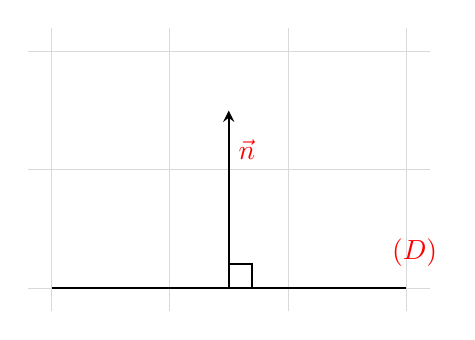
\begin{tikzpicture}[scale=1.5, >=stealth]
    % Grille de fond (lignes grises fines comme sur un cahier)
    \draw[help lines, color=gray!30, solid] (-1.2,-0.2) grid (2.2,2.2);

    % Dessin de la droite horizontale (en noir)
    \draw[thick] (-1,0) -- (2,0);

    % Dessin du vecteur normal n (en noir, mais labellisé en rouge)
    \draw[->, thick] (0.5,0) -- (0.5,1.5);
    
    % Marquage de l'angle droit (petit carré en noir)
    \draw[thick] (0.5,0.2) -- (0.7,0.2) -- (0.7,0);

    % Label du vecteur n (en rouge, au-dessus de la flèche)
    \node[anchor=south west, color=red] at (0.5,1) {$\vec{n}$};

    % Label de la droite (D) (en rouge, à droite)
    \node[anchor=west, color=red] at (1.8,0.3) {$(D)$};

\end{tikzpicture}
\end{center}

\noindent \underline{\textcolor{red}{Exemples :}}

\begin{enumerate}
    \item $(D) : 2x + 3y + 1 = 0$ ($a = 2$, $b = 3$ et $c = 1$) \\
    $\vec{u} \begin{pmatrix} -3 \\ 2 \end{pmatrix}$ est un vecteur directeur de $(D)$. \\
    $\vec{n} \begin{pmatrix} 2 \\ 3 \end{pmatrix}$ est un vecteur normal de $(D)$.
    
    \item $(D') : 3x + 5 = 0$ ($a = 3$, $b = 0$ et $c = 5$) \\
    $\vec{u} \begin{pmatrix} 0 \\ 3 \end{pmatrix}$ est un vecteur directeur de $(D')$. \\
    $\vec{n} \begin{pmatrix} 3 \\ 0 \end{pmatrix}$ est un vecteur normal de $(D')$.
    
    \item $(\Delta) : -y + 8 = 0$ ($a = 0$, $b = -1$, $c = 8$) \\
    $\vec{u} \begin{pmatrix} 1 \\ 0 \end{pmatrix}$ est un vecteur directeur de $(\Delta)$. \\
    $\vec{n} \begin{pmatrix} 0 \\ -1 \end{pmatrix}$ est un vecteur normal de $(\Delta)$.
\end{enumerate}

\noindent \underline{\textcolor{red}{Propriété}} \\
Soient : $(D) : ax + by + c = 0$ \\
\indent \qquad $(D') : a'x + b'y + c' = 0$ \\
où $a, b, c, a', b', c'$ des réels tels que : $(a, b) \neq (0, 0)$ et $(a', b') \neq (0, 0)$.

\begin{itemize}
    \item[i)] \textcolor{red}{$(D) // (D')$} si \textcolor{red}{$ab' - a'b = 0$}
    \item[ii)] \textcolor{red}{$(D) \perp (D')$} si \textcolor{red}{$aa' + bb' = 0$}
\end{itemize}

\noindent \underline{\textcolor{red}{Remarque :}} \\
Soit $(D) : ax + by + c = 0$ où $a, b, c$ des réels avec $(a, b) \neq (0, 0)$
\begin{itemize}
    \item[i)] \textcolor{red}{$(D) // (xx')$} ssi \textcolor{red}{$a = 0$}
    \item[ ] \textcolor{red}{$(D) // (yy')$} ssi \textcolor{red}{$b = 0$}
\end{itemize}

\vspace{0.5cm}

\subsection*{\underline{\textcolor{red}{b) Équation réduite d'une droite}}}

\noindent \underline{\textcolor{red}{Définition :}} \\
L'équation \textcolor{red}{réduite} d'une droite est de la forme \textcolor{red}{$y = mx + p$} où $m$ et $p$ des réels.
\begin{itemize}
    \item \textcolor{red}{$m$} est appelé \textcolor{red}{coefficient directeur} de $(D)$.
    \item \textcolor{red}{$p$} est appelé \textcolor{red}{l'ordonnée à l'origine}.
\end{itemize}

% --- Propriété : Positions relatives ---

\noindent \underline{\textcolor{red}{Propriété :}} Soient $(D) : y = mx + p$ où $m, p \in \mathbb{R}$ \\
\indent \qquad \qquad \qquad $(D') : y = m'x + p$ où $m', p \in \mathbb{R}$

\begin{itemize}
    \item[i)] \textcolor{red}{$(D) // (D')$} ssi \textcolor{red}{$m = m'$}
    \item[ii)] \textcolor{red}{$(D) \perp (D')$} ssi \textcolor{red}{$mm' = -1$}
\end{itemize}

\vspace{0.5cm}

\begin{center}
    \underline{\textcolor{red}{Application}}
\end{center}

\noindent On considère l'ensemble $(D_m)$ des points $M \begin{pmatrix} x \\ y \end{pmatrix}$ vérifiant : \\
$(m-1)x + (2m+1)y + 3 = 0$ (où $m$ est un paramètre réel).

\begin{enumerate}
    \item Montrer que $(D_m)$ est une droite du plan pour tout réel $m$.
    \item Montrer que toutes les droites $(D_m)$ passent par un point fixe $A$ que l'on précisera.
    \item Pour quelle(s) valeur(s) de $m$, la droite $(D_m)$ est parallèle à :
    \begin{itemize}
        \item[a)] l'axe des abscisses
        \item[b)] l'axe des ordonnées
        \item[c)] À la droite $(\Delta) : x + 2y + 1 = 0$
    \end{itemize}
    \item Pour quelle(s) valeur(s) de $m$, la droite $(D_m)$ est perpendiculaire à la droite $(D') : 3x + 4y + 1 = 0$
\end{enumerate}

% --- Correction de l'Application (Droites Dm) ---

\begin{center}
    \underline{\textcolor{red}{Correction de l'Application}}
\end{center}

On considère $(D_m) : (m-1)x + (2m+1)y + 3 = 0$.

\begin{enumerate}
    \item \textbf{Montrons que $(D_m)$ est une droite pour tout réel $m$ :}
    Une équation de la forme $ax + by + c = 0$ est une droite si $(a, b) \neq (0, 0)$.
    Ici, $a = m-1$ et $b = 2m+1$.
    Cherchons si $a$ et $b$ peuvent être nuls simultanément :
    $m-1 = 0 \Rightarrow m = 1$.
    Si $m=1$, alors $b = 2(1)+1 = 3 \neq 0$.
    Les coefficients ne sont jamais nuls en même temps, donc \textcolor{red}{$(D_m)$ est toujours une droite}.

    \item \textbf{Montrons que toutes les droites passent par un point fixe $A$ :}
    Développons l'équation par rapport à $m$ :
    $mx - x + 2my + y + 3 = 0$
    $m(x + 2y) + (-x + y + 3) = 0$
    Pour que cette égalité soit vraie quel que soit $m$, il faut :
    \[ \begin{cases} x + 2y = 0 \quad (1) \\ -x + y + 3 = 0 \quad (2) \end{cases} \]
    De (1), on a $x = -2y$. En remplaçant dans (2) :
    $-(-2y) + y + 3 = 0 \Rightarrow 3y = -3 \Rightarrow y = -1$.
    D'où $x = -2(-1) = 2$.
    Toutes les droites passent par le point fixe \textcolor{red}{$A \begin{pmatrix} 2 \\ -1 \end{pmatrix}$}.

    \item \textbf{Valeurs de $m$ pour le parallélisme :}
    Le vecteur normal de $(D_m)$ est $\vec{n} \begin{pmatrix} m-1 \\ 2m+1 \end{pmatrix}$.
    \begin{itemize}
        \item[a)] \textbf{Axe des abscisses ($y=0$)} : La droite doit être de la forme $y = k$, donc le coefficient de $x$ doit être nul.
        $m-1 = 0 \Rightarrow \textcolor{red}{m = 1}$.
        \item[b)] \textbf{Axe des ordonnées ($x=0$)} : La droite doit être de la forme $x = k$, donc le coefficient de $y$ doit être nul.
        $2m+1 = 0 \Rightarrow \textcolor{red}{m = -1/2}$.
        \item[c)] \textbf{Parallèle à $(\Delta) : x + 2y + 1 = 0$} :
        Condition $ab' - a'b = 0$ :
        $(m-1)(2) - (1)(2m+1) = 0$
        $2m - 2 - 2m - 1 = -3$.
        $-3 \neq 0$, donc \textcolor{red}{aucune valeur de $m$} ne rend $(D_m)$ parallèle à $(\Delta)$.
    \end{itemize}

    \item \textbf{Perpendicularité avec $(D') : 3x + 4y + 1 = 0$ :}
    Condition $aa' + bb' = 0$ :
    $3(m-1) + 4(2m+1) = 0$
    $3m - 3 + 8m + 4 = 0$
    $11m + 1 = 0 \Rightarrow \textcolor{red}{m = -1/11}$.
\end{enumerate}
\textbf{\underline{\exemple}}

\textbf{\underline{\solution}}        
        
\textbf{\underline{\exerciceapp}}

\textbf{\underline{\correction}}

\end{document}
